\begin{figure}

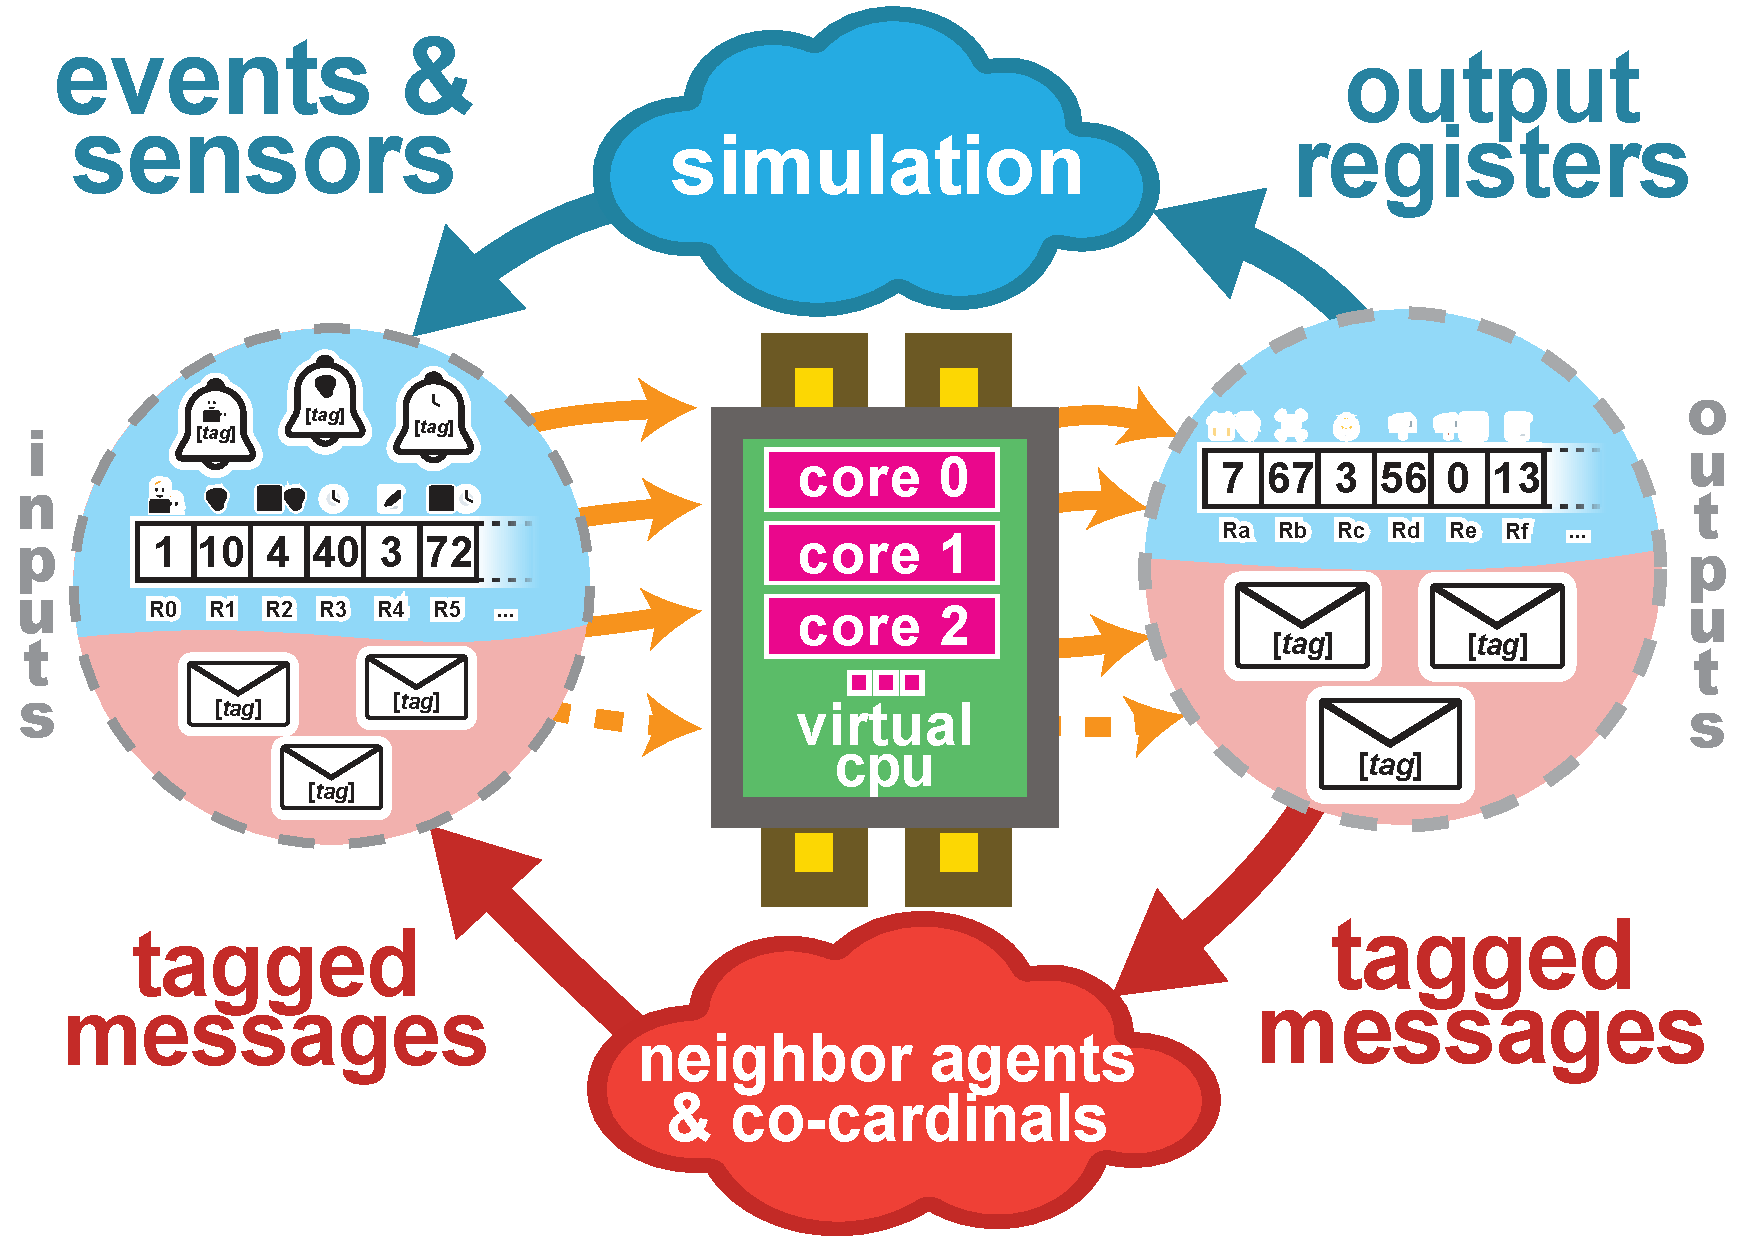
\includegraphics[width=\linewidth]{{img/cpu_detail}}

\caption{
\textbf{Overview of genome execution.}
\footnotesize
Tagged events and messages (shown as bells and envelopes, respectively) activate module execution on virtual cores.
Simulation state can also be read directly using sensor instructions to access input registers.
Special instructions write to output registers, allowing interaction with the simulation, and generate tagged messages, allowing interaction with other virtual CPUs.
}
\label{fig:cpu_detail}
\end{figure}
